\documentclass{lecturenotes}

\newcommand{\DateOfShow}{2020-08-26}
\newcommand{\Startdag}{måndag}
\newcommand{\KursStartTidDod}{kl 10:15 Online}
\newcommand{\KursStartTidPgk}{kl 13:15 Hybrid (E:A+Online)}

\title[Kort presentation av pgk \& dod, \DateOfShow]{\textbf{EDAA45} Programmering, grundkurs (pgk) \\ + \\ \textbf{EDAA60} Datorer och datoranvändning (dod)}
\author{\href{http://cs.lth.se/bjorn-regnell}{Björn Regnell}, \href{http://cs.lth.se/per-andersson/}{Roger Henriksson}}
\institute{\href{http://cs.lth.se}{Datavetenskap}, LTH}
\date{\DateOfShow}

\begin{document}

\frame{\titlepage}

\frame{\frametitle{En kurskombo som startar på \Startdag}
Lägger grunden för alla kommande kurser i datavetenskap: \vspace{1em}
\begin{itemize}
  \item \Alert{Programmering, grundkurs} (pgk), 7.5 hp, 16 veckor
  \begin{itemize}
    \item[] En grundlig genomgång av programmering \Emph{från början} \\ med stora möjligheter till \Emph{fördjupning} som du själv väljer
  \end{itemize}
  \vspace{1em}
  \item \Alert{Datorer och datoranvändning} (dod), 3 hp, 3 veckor
  \begin{itemize}
    \item[] Inblick i hur datorer fungerar och verktygen vi använder
  \end{itemize}
\end{itemize}
}

\frame{\frametitle{Vad ska du lära dig?}
%Att skapa koden som styr världen...
%\includegraphics[width=1.2\textwidth, height=1.5cm]{img/code-wide}
\begin{multicols}{2}
\begin{itemize}\Size{9pt}
\item \textbf{Programmering, grundkurs}
\begin{itemize}\Size{8pt}
\item Tänka i abstraktioner
\item Använda datastrukturer
\item Implementera algoritmer
\item Brepp som lägger grunden för resten av din utbildning
\item Språk: \Emph{Scala} (och lite Java)
\end{itemize}
\columnbreak
\item \textbf{Datorer \& datoranvändning}
\begin{itemize}\Size{8pt}
\item Lågnivåprogrammering
\item Datarepresentation
\item Terminalkommando i Linux
\item Skriva \& typsätta i \LaTeX
\item Beräkningar i Matlab
\end{itemize}
\end{itemize}
\end{multicols}
\vspace{2em}
\flushright\scriptsize Denna presentation i \LaTeX\ på GitHub:
\\{\tiny\url{https://github.com/lunduniversity/introprog/blob/master/slides/info-week00.tex}}
}

%%%
\frame{\frametitle{Hur ska du lära dig?}
\begin{itemize}
\item Genom praktiskt eget arbete: Lära genom att göra!
\begin{itemize}
\item Övningar
\item Laborationer
\item Projekt
\end{itemize}
\item Genom studier av viktiga begrepp: Skapa förståelse på djupet och lägga bred grund för din fortsatta utbildning
\item Genom samarbete med dina kurskamrater
\end{itemize}
}

%%%
% \frame{\frametitle{Kurslitteratur}
% \footnotesize
% \begin{columns}
% \begin{column}{0.65\textwidth}
% {\Size{16pt}pgk:}
% \begin{itemize}
% \item 2 st kompendier 358+360 sidor \\ Säljs till självkostnadspris på institutionen. \\ Beställ bokpaket om du inte redan gjort det här \Alert{senast idag kl 12} för mängdrabatt: \url{http://cs.lth.se/pgk/bokpaket}
% \end{itemize}
% \vspace{1em}
% {\Size{16pt}dod:}
% \begin{itemize}
% \item Kursmaterial delas ut på första föreläsningen.
% \end{itemize}
% \end{column}
% \begin{column}{0.35\textwidth}
% \centering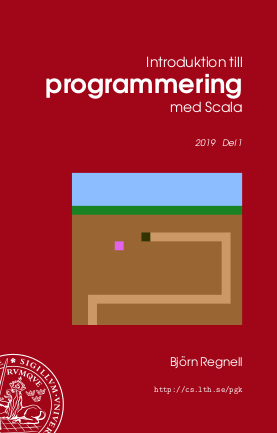
\includegraphics[width=0.99\textwidth]{../img/compendium-front-page-2019.png}
% \end{column}
% \end{columns}
% }

\begin{Slide}{Bokpaket}
  \begin{itemize}
    %\item Det är 117 D-are, 4 W-are och 4 fristående som beställt kursmaterial. Grattis! :)
    \item D:are får bokpaket mot uppvisande av Swish-transaktion via faddrar:
    \item[] *** Swishnummer: 123 170 4584
    \item[] *** Ange meddelande: pgk <förnamn efternamn>
    \item[] *** Belopp: 455 kr 
    \item D-are som missat fadderutdelningen samt W:are och fristående hämtar på cs expedition under expeditionstider mot uppvisande av Swish-transaktion enl ovan.
    \item Efterbeställning möjlig via Canvas. De första 10 får lägre priset därefter högre priset.
  \end{itemize}
\end{Slide}




\SlideImg{Stor spridning i förkunskaper}{../img/survey-2020}


\begin{Slide}{Andelen D-are som vid kursstart aldrig kodat}
\pgfplotstableread[row sep=\\,col sep=&]{
    år & nybörjare\\
    2015 & 19  \\
    2016 & 32  \\
    2017 & 38  \\
    2018 & 31  \\
    2019 & 30  \\
    2020 & 20  \\
    }\dataSeq

\begin{minipage}{0.65\textwidth}
\hspace*{-0.65cm}%
\begin{tikzpicture}[scale=0.9, every node/.style={scale=0.9}]
    \begin{axis}[
            ybar,
            bar width=1.0cm,
            symbolic x coords={2015,2016,2017,2018,2019,2020},
            xtick=data,
            nodes near coords,
            nodes near coords align={vertical},
            legend style={at={(0.5,1)},anchor=south,legend columns=-1,draw=none},
            ymin=0,ymax=45,
            ylabel={\%},
            xlabel={År},
        ]
        \addplot table[x=år,y=nybörjare]{\dataSeq};
        %\legend{nybörjare}
    \end{axis}
\end{tikzpicture}
\end{minipage}%
\begin{minipage}{0.3\textwidth}
\begin{itemize}\SlideFontTiny
\item[] År: antal enkätsvar D
\item[] 2015: 102 st
\item[] 2016: 104 st
\item[] 2017: 114 st
\item[] 2018: 123 st
\item[] 2019: 125 st 
\item[] 2020: 137 st 
\end{itemize}
\end{minipage}%
\end{Slide}


%%%

\frame[plain]{\frametitle{Beställ bokpaket!}
Bokpaketet är \Emph{fantastiskt!}\\~\\
\url{http://cs.lth.se/pgk/bokpaket}\\~\\
\Alert{Om du inte fyllt i den gör det nu!}\\ (Även om du svarar ''Nej'')
}

\frame[plain]{\frametitle{Förkunskapsenkät}

Ditt svar på denna \Emph{förkunskapsenkät} används i planeringen:
\url{http://cs.lth.se/pgk/introsurvey}\\
\Alert{Om du inte fyllt i den gör det nu!}\\
\vspace{1em}
Enkäten innehåller dessa frågor och några till:
\begin{itemize}
\item Har du programmerat tidigare? \\
         Ja \hspace{2.5cm} Nej
\item Hur många program har du skrivit? \\
         $<5$ \hspace{2.2cm} $5-20$ \hspace{2.5cm}  $>20$
\item Hur stort var det största program du har skrivit?\\
         $<50$ rader \hspace{1cm} $50 - 500$  rader \hspace{1cm}  $>500$ rader
\end{itemize}
\vspace{1em}
}




\frame{\frametitle{Välkommen till kursupprop på \Startdag!}
I matte-annexet (MA):
\begin{itemize}
\item  dod: \KursStartTidDod 
\item  pgk: \KursStartTidPgk
\item[] 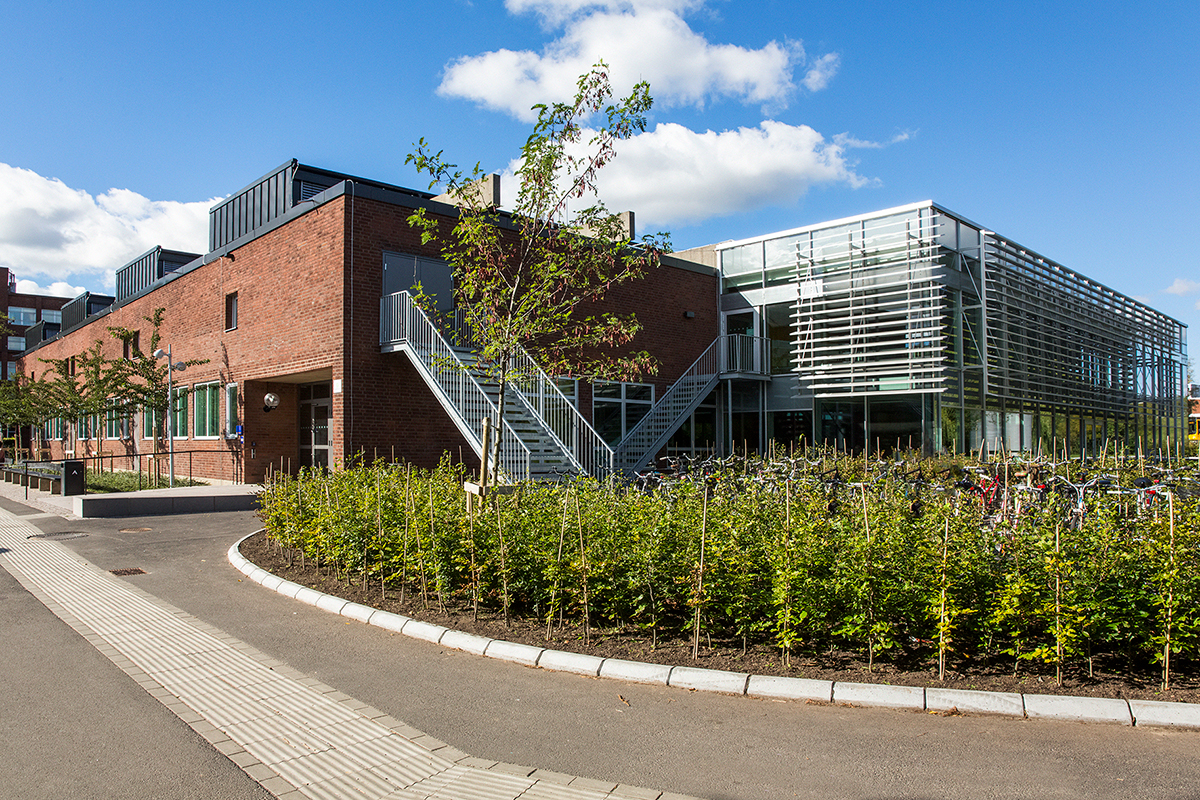
\includegraphics[height=0.41\textheight]{../img/annexet}
\end{itemize}

Besök kurshemsidorna för mer information: 
\begin{itemize}
  \item \url{http://cs.lth.se/pgk} 
  \item \url{http://cs.lth.se/dod}
\end{itemize}

}

\end{document}
